\chapter{ANALISIS DAN PERANCANGAN}

\section{Model Desain}
    Secara garis besar, topik ini akan dibagi menjadi dua buah subsistem yang lebih kecil yakni \textit{resource allocator} dan \gls{dds}.
    Penjelasan lebih lanjut mengenai rincian desain subsistem dan pembagian kerja akan dibahas pada tabel \ref{tab:subsistemDivision}.

    \begin{table}[tbh]
        \caption{Pembagian Subsistem}\label{tab:subsistemDivision}
        \begin{center}
            \begin{tabular}{|m{0.5cm}|m{3cm}|m{5.5cm}|m{3cm}|}
                \hline
                \thead{No} & \thead{Subsistem} & \thead{Rincian Desain Subsistem} & \thead{Pembagian Kerja}\\
                \hline 
                1 & \textit{Resource Allocator} & \textit{Resource Allocator} berperan untuk melakukan alokasi \textit{bandwidth} secara tepat dan efisien yang bertujuan untuk meningkatkan rata-rata akurasi dari sistem \gls{vap} & Faishal Zharfan \\
                \hline 
                2 & \gls{dds} & \gls{dds} berperan dalam optimasi pengaturan konfigurasi parameter pengkodean dan kompresi video untuk mencapai akurasi inferensi terbaik. & Farhan Krishna\\
                \hline 
            \end{tabular}
        \end{center}
    \end{table}
    
    \subsection{\textit{Resource Allocator}}

        \begin{figure}[tbh]
            \centering
            \includesvg[scale=0.45]{./resources/resourceAlloc_simple.svg}
            \caption{Resource Allocator Simple}\label{fig:resourceAllocSimple}
        \end{figure}

        Secara umum, \textit{resource allocator} yang akan didesain memiliki alur kerja seperti pada gambar \ref{fig:resourceAllocSimple} di atas. 
        Terdapat 4 proses utama yakni \textit{Initialization}, \textit{Profiling}, \textit{Optimization}, dan \textit{Allocation}.
        \textit{Initialization} adalah sebuah proses ketika \textit{resource allocator} pertama kali dijalankan, pada proses ini \textit{resource allocator} akan membaca parameter-parameter yang didefinisikan, menyiapkan \textit{port} komunikasi, dan memulai \textit{agent} pada \textit{background} sebagai \gls{api}.
        Pada proses ini pula para klien \gls{vap} akan melakukan proses \textit{check-in} dan menjalin komunikasi dengan \textit{resource allocator} menggunakan \gls{api} gRPC, dan tahapan terakhir adalah pembagian bandwidth kepada masing-masing \gls{vap}.

        \textit{Resource allocator} akan berada dalam kondisi \textit{idle} atau menunggu hingga proses \textit{Profiling} tiba. Proses ini akan meminta para \gls{vap} yang terhubung untuk menaikan dan menurunkan \textit{bandwidth}-nya masing-masing dan melakukan \textit{inference} terhadap \textit{bandwidth} tersebut.
        Setelahnya, hasil deteksi objek kedua \textit{bandwidth} akan diperoleh, kedua hasil ini akan dibandingkan dengan hasil deteksi objek pada \textit{bandwidth} saat ini, hasil ini lah yang dinamakan \textit{inferDiff}. \textit{inferDiff} inilah yang kemudian akan dikirim kepada \textit{resource allocator}
        untuk selanjutnya diproses dan dilakukan penentuan alokasi \textit{bandwidth}.

        Setibanya \textit{inferDiff} pada \textit{resource allocator}, proses selanjutnya adalah \textit{Optimization}. Pada proses ini, \textit{inferDiff} akan diolah sedemikian sehingga tiap \textit{inferDiff} menjadi sebuah persamaan garis yang dependen satu sama lainnya
        dan akan dijalankan algoritma \textit{linear programming} untuk menentukan besaran alokasi \textit{bandwidth} terbaik untuk tiap klien \gls{vap}.
        Selanjutnya hasil \textit{Optimization} akan berupa alokasi \textit{bandwidth} yang sesuai dengan kebutuhan \gls{vap}. \textit{Allocation} akan mengirimkan notifikasi kepada tiap \gls{vap} terkait alokasi \textit{bandwidth} yang mereka dapatkan.
        Lebih lengkap terkait implementasi proses-proses tersebut akan dibahas pada bagian selanjutnya.

\section{Implementasi}
    \subsection{Initialization}

        \begin{figure}[tbh]
            \centering
            \includesvg[scale=0.5]{./resources/init.svg}
            \caption{Initialization Flow Chart}\label{fig:initialization}
        \end{figure}    

        Proses \textit{Initialization} secara umum dapat dilihat pada gambar \ref{fig:initialization}. Proses pertama yang dilakukan adalah \textit{parameter loading}, yakni membaca parameter yang terdapat pada program \textit{runResourceAllocator.sh} seperti pada Lampiran A.
        Secara singkat, parameter-parameter yang digunakan adalah seperti berikut ini.

        \begin{itemize}
            \item \textbf{bandwidth} (Kbps)
            \item \textbf{monitorInterval} (detik) 
            \item \textbf{bandwidthDelta} (Kb)
        \end{itemize}

        Parameter \textbf{bandwidth} digunakan untuk menentukan seberapa banyak \textit{bandwidth} total yang ingin digunakan dalam sistem, dalam satuan Kbps.
        Sementara parameter \textbf{monitorInterval} menandakan periode \textit{profiling} atau pengalokasian bandwidth, dapat dikatakan bahwa \textbf{monitorInterval} mengatur berapa lama jarak antar \textit{profiling} terjardi. 
        Terakhir, parameter \textbf{bandwidthDelta} menandakan berapa seberapa banyak bandwidth yang ingin dialokasikan dari satu video ke video yang lain dalam satu kali iterasi \textit{profiling}.

        \begin{algorithm}[tbh]
        \caption{Algoritma \textit{Port Initialization}}\label{alg:portInit}
        \textit{\textbf{import} grpc, threadExec}
        \begin{algorithmic}[1]
            \Procedure{initServer}{$workerNumber$}
                \State $srv \gets grpc.server(threadExec(workerNumber))$
                \State $srv.addPort("0.0.0.0:5000")$
                \State $srv.start()$
                \State $srv.waitForTermination()$
            \EndProcedure
        \end{algorithmic}
        \end{algorithm}

        Tahapan selanjutnya adalah \textit{port initialization} yang \textit{pseudocode} dapat dilihat pada \textit{pseudocode} \ref{alg:portInit}. Setelah pembacaan parameter, selanjutnya 
        \textit{resource allocator} akan dijalankan. Pada tahap ini program membutuhkan variabel \textbf{workerNumber} yang berguna untuk menginformasikan seberapa banyak \gls{vap} maksimal yang bisa terhubung.
        satu \gls{vap} yang terhubung akan memiliki kanal komunikasi sendiri dengan \textit{resource allocator}. \textit{Resource allocator} akan dijalankan pada \textbf{port 5000}, sehingga ketika 
        sebuah \gls{vap} ingin terhubung dengan \textit{resource allocator}, mereka dapat menghubungi \textit{port} tersebut. Selanjutnya servis dari \textit{resource allocator} akan dihidupkan hingga terdapat \textit{termination}.

        \begin{algorithm}[tbh]
        \caption{Algoritma \textit{Client Check-in}}\label{alg:appCheckin}
        \begin{algorithmic}[1]
        \Procedure{clientCheckin}{$clentRequest$}
        \State $NumApps \gets NumApps + 1$
        \State $bandwidthAllocation \gets MaxBW/NumApps$ \Comment{In Kbps}
        \State $app \gets PipelineRepr(clientRequest)$
        \State $clients.add(app)$
        \For{$client$ in $clients$}
        \State $client.limit(bandwidthAllocation)$
        \State $client.notify(bandwidthAllocation)$
        \EndFor
        \EndProcedure
        \end{algorithmic}
        \end{algorithm}

        Proses selanjutnya adalah \textit{client check-in}, pada proses ini, \gls{vap} akan melakukan \textit{check-in} kepada \textit{resource allocator} untuk mendapatkan alokasi \textit{bandwidth}. Selain itu, \gls{vap}
        yang sudah terhubung sebelumnya akan mendapat penyesuaian jumlah \textit{bandwidth}, hal ini akan terus berlangsung hingga tidak ada \gls{vap} yang melakukan \textit{check-in} lagi.
        Pada kondisi ini, baik \textit{resource allocator} maupun \gls{vap} sudah saling terhubung dan dapat berkomunikasi satu sama lain. Perhatikan bahwa \textit{resource allocator} memiliki fungsi \textit{limit()}, fungsi 
        ini diimplementasikan menggunakan TC dan berguna untuk melimitasi \textit{data rate} yang masuk kepada \textit{server}. Sehingga setiap \gls{vap} memiliki \textit{inbound interface}-nya masing-masing pada server dan dilimitasi mengikuti ukuran \textit{bandwidth}-nya.

    \subsection{Profiling}\label{sec:profiling}

        \begin{figure}[tbh]
            \centering
            \includesvg[scale=0.5]{./resources/profiling.svg}
            \caption{Initialization Flow Chart}\label{fig:profiling}
        \end{figure} 

        Tahapan kedua adalah \textit{Profiling}. Pada tahapan ini akan terjadi interaksi antara \textit{resource allocator} dan \gls{vap}. Proses-proses yang terlibat dapat dilihat pada gambar \ref{fig:profiling}. 

        \begin{algorithm}[tbh]
        \caption{Algoritma notify clients}\label{alg:notifyClients}
        \begin{algorithmic}[1]
        \Procedure{notifyClients}{$bandwidthDelta$}
        \For{$client$ in $clients$}
        \State $client.prepareProfiling(bandwidthDelta)$
        \EndFor
        \State $waitForAllACK()$
        \EndProcedure
        \end{algorithmic}
        \end{algorithm}

        Tahapan selanjutnya adalah \textit{notify clients}, \textit{pseudocode} mengenai proses ini adalah seperti tertera pada algoritma \ref{alg:notifyClients}. Pada \textit{notify clients}, \textit{resource allocator} akan memberi notifikasi kepada \gls{vap} untuk bersiap-siap melakukan \textit{profiling}.  
        Notifikasi yang diberikan termasuk pemberian informasi mengenai seberapa
        besar \textit{bandwidthDelta} yang diberikan. Setelah diberikan notifikasi, \gls{vap} akan menunggu hingga proses \textit{inference} atau deteksi objek pada segmen video saat ini untuk selesai dan siap untuk proses \textit{profiling} dengan memberi notifikasi kepada \textit{resource allocator}.

        \begin{algorithm}[tbh]
            \caption{Algoritma getInferdiff Client}\label{alg:getInferdiffClient}
            \begin{algorithmic}
                \Procedure{getInferDiff}{}
                \For{$client$ in $clients$}
                \State $client.getInferDiff()$
                \EndFor
                \EndProcedure
            \end{algorithmic}
        \end{algorithm}

        \begin{algorithm}[tbh]
            \caption{Algoritma getInferdiff Server}\label{alg:getInferdiffServer}
            \begin{algorithmic}
                \Ensure $inferDiff$
                \Procedure{getInferDiff}{}
                \State $currentBW \gets currentBW + deltaBW$
                \State $changeToBestConfig(currentBW)$
                \State $highResult \gets analyzeVideo()$
                \State $highInferDiff \gets evaluate(highResult)$
                \State $currentBW \gets currentBW - 2 * deltaBW$
                \State $changeToBestConfig(currentBW)$
                \State $lowResult \gets analyzeVideo()$
                \State $lowInferDiff \gets evaluate(lowResult)$
                \State $sendToServer(highInferDiff,\ lowInferDiff)$
                \EndProcedure
            \end{algorithmic}
        \end{algorithm}


        Hal ini berlanjut kepada proses selanjutnya yakni \textit{get inferdiff}. Terdapat 2 \textit{pseudocode} yang ditampilkan, yakni \textit{pseudocode} pada \textit{server} seperti terlihat pada \ref{alg:getInferdiffServer} dan \textit{client} seperti terlihat pada \ref{alg:getInferdiffServer}.
        Pada \textit{pseudocode} \ref{alg:getInferdiffServer}, \textit{server} akan men-\textit{trigger} \textit{client} untuk melakukan \textit{profiling}. Sementara pada \textit{client}, tahapan yang terjadi adalah sebagai berikut.
        Klien \gls{vap} akan menaikan \textit{bandwidth} berdasarkan \textit{deltaBandwidth} yang sudah ditetapkan sebelumnya. Selanjutnya \gls{vap} akan mengubah konfigurasi segmen video berdasarkan \textit{bandwidth} tersebut.
        Konfigurasi video yang dimaksud adalah sebagai berikut

        \begin{enumerate}
            \item \textbf{Quantization Parameter (QP)}
            \item \textbf{Resolution}
            \item \textbf{Entropy}
            \item \textbf{Directional Prediction}
            \item \textbf{Partition Size}
            \item \textbf{Motion Estimation}
        \end{enumerate}

        Selanjutnya segmen video tersebut akan dianalisis atau dilakukan deteksi objek berdasarkan konfigurasi tersebut. Setelah analisis selesai dilakukan, \textit{inferDiff} akan dihitung, perhitungan mengenai hal ini akan dibahas lebih
        lanjut pada \ref{sec:inferDiff}. Lalu \gls{vap} akan menurunkan \textit{bandwidth}-nya, persis seperti sebelumnya, konfigurasi video akan diubah kembali, dilakukan deteksi objek, dan \textit{inferDiff} akan dihitung kembali. Pada akhirnya
        akan diperoleh 2 hasil, yakni \textit{inferDiff} saat \textit{bandwidth} dinaikan dan diturunkan. Kedua hasil inilah yang akan dikirim kembali kepada \textit{resource allocator} untuk diproses lebih lanjut untuk diperoleh alokasi \textit{bandwidth} yang optimal.

        \subsubsection{inferDiff}\label{sec:inferDiff}

        \textit{inferDiff} adalah sebuah satuan yang digunakan untuk mengukur seberapa sensitif sebuah \gls{vap} terhadap perubahan bandwidth atau dikenal dengan \textit{sensitivity}. Pada keadaan ideal, pengukuran \textit{sensitivity}
        adalah selisih dari akurasi pada \textit{bandwidth} saat ini dan \textit{bandwidth} saat dinaikan (\textit{lowSensitivity}) maupun diturunkan (\textit{highSensitivity}). 
        Sehingga \textit{pseudocode}-nya adalah seperti tertera pada \ref{alg:calcF1}

        \begin{algorithm}[tbh]
        \caption{Algoritma Kalkulasi \textit{Sensitivity}}\label{alg:calcF1}
        \begin{algorithmic}[1]
        \Procedure{sensitivityCalculation}{}
        \Function{calcF1}{$result,\ gt$}
            \State $f1Score \gets eval(result,\ gt)$
            \State \textbf{return} $f1Score$
        \EndFunction
        \State $highSensitivity \gets calcF1(highRes,\ gt) - calcF1(currRes,\ gt)$
        \State $lowSensitivity \gets calcF1(currRes,\ gt) - calcF1(lowRes,\ gt)$
        \State $Sensitivity \gets (lowSensitivity,\ highSensitivity)$
        \EndProcedure
        \end{algorithmic}
        \end{algorithm}

        Pada \textit{pseudocode} \ref{alg:calcF1} tersebut, terdapat variabel \textbf{gt} atau \textit{ground truth}. \textit{Ground truth} adalah sebuah hasil hasil deteksi objek
        pada keadaan yang sesungguhnya, maksudnya adalah ketika kita ingin menghitung akurasi atau \textit{f1-score} dari sebuah model objek deteksi, hasil deteksi harus dibandingkan
        dengan video yang memiliki kualitas yang sangat baik. Hal ini mustahil untuk dilakukan karena \textit{ground truth} tidak mungkin diketahui pada saat program berjalan.

        \begin{algorithm}[tbh]
        \caption{Algoritma Kalkulasi inferDiff}\label{alg:inferDiff}
        \begin{algorithmic}[1]
        \Procedure{inferDiffCalculation}{}
        \Function{calcF1}{result, gt}
            \State $f1Score \gets eval(result,\ gt)$
            \State \textbf{return} $f1Score$
        \EndFunction
        \State $highinferDiff \gets 1 - calcF1(currRes,\ highRes)$
        \State $lowinferDiff \gets 1 - calcF1(lowRes,\ currRes)$
        \State $inferDiff \gets (lowinferDiff,\ highinferDiff)$
        \EndProcedure
        % \Comment{currRes = currentRes, highRes = highResult, lowRes = lowResult}
        \end{algorithmic}
        \end{algorithm}

        Oleh karena hal itu, dirumuskanlah sebuah istilah baru, yakni \textit{inferDiff}.
        Berbeda dengan \textit{oracle}-nya yang membutuhkan \textit{ground truth}, \textit{inferDiff} akan memperlakukan hasil deteksi sebagai \textit{ground truth} relatif. Sebagai contoh, \textbf{highResult} merupakan \textit{ground truth} relatif terhadap \textbf{currentResult}
        dan \textbf{currentResult} sebagai \textit{ground truth} relatif terhadap \textbf{lowResult} sehingga perhitungannya adalah seperti tertera pada \textit{pseudocode} \ref{alg:inferDiff}
        Walaupun tidak ideal, metode perhitungan \textit{inferDiff} ini berkolerasi positif terhadap perhitungan \textit{sensitivity} yakni ketika \textit{ground truth}-nya diketahui. 
        Sehingga \textit{inferDiff} dapat digunakan pada sistem yang \textit{real-time}.


    \subsection{Optimization}

        \begin{figure}[tbh]
            \centering
            \includesvg[scale=0.4]{./resources/optimization.svg}
            \caption{Optimization}\label{fig:optimization}
        \end{figure} 

        Proses selanjutnya adalah \textit{optimization}, pada bagian ini akan dilakukan perhitungan dan penentuan atas \gls{vap} mana saja yang berhak untuk 
        memperoleh alokasi \textit{bandwidth} dan \gls{vap} mana yang perlu dikurangi. Secara umum, tahapan yang terjadi adalah seperti tertera pada gambar \ref{fig:optimization}. 
        Proses ini memerlukan masukan \textit{inferDiff} yang telah diperoleh pada tahapan sebelumnya (\ref{sec:profiling}). 
        Selanjutnya, \textit{inferDiff} yang diperoleh akan diproses sedemikian rupa sehingga datanya 
        dependen antara satu \gls{vap} dengan \gls{vap} lainnya. Lalu, dari hasil tersebut akan dilakukan pemrosesan lebih lanjut sehingga diperoleh
        pertidaksamaan yang akan dipecahkan atau diselesaikan dengan teknik \textit{linear optimizatioin} atau dikenal dengan \textit{linear programming} sehingga dapat ditentukan \gls{vap} mana yang membutuhkan \textit{bandwidth} lebih dan mana yang dapat dikurangi.

        \begin{algorithm}[tbh]
        \caption{Algoritma \textit{Victim Determination}}\label{alg:victimDetermination}
        \begin{algorithmic}[1]
        % \Require $test$
        \Procedure{victimDetermination}{$void$}
        \State $victim \gets None$
        \State $victimHigh \gets 1$
        \State $victimLow \gets -1$
        \For{$client$ in $clients$}
        \If{$client.lowinferDiff \geq victimLow$}
        \If{$client.highinferDiff \leq victimhigh$}
        \If{$client.isNotMinBW$}
        \State $victim \gets client$
        \EndIf
        \EndIf
        \EndIf
        \EndFor
        \EndProcedure
        \end{algorithmic}
        \end{algorithm}

        Sebelum memroses data \textit{inferDiff}, perlu ditentukan terlebih dahulu siapa yang jadi korban atau \textit{victim}. Algoritma terkait pemilihan \textit{victim} dapat dilihat pada \textit{pseudocode} \ref{alg:victimDetermination}.
        Dalam hal ini, \textit{victim} adalah sebuah \gls{vap} yang memiliki \textbf{lowinferDiff} yang paling tinggi dan \textbf{highinferDiff} yang paling rendah
        serta tidak berada pada \textit{bandwidth} minimal, artinya \textit{bandwidth}-nya bisa dikurangi. Dengan demikian, \textit{victim} adalah sebuah \gls{vap} yang \textit{bandwidthnya} akan dikurangi dan dialokasian kepada \gls{vap} lain


        \begin{algorithm}[tbh]
        \caption{Algoritma \textit{Optimizing}}\label{alg:optimizing}
        \begin{algorithmic}[1]
        % \Require $test$
        \Procedure{optimizing}{$void$}
        \For{$client$ in $clients$}
        % \State $client.prepareProfiling(bandwidthDelta)$
        \State $client.sensitivity \gets client.highinferDiff - victimLow$
        % \For{$enemy$ in $clients$}
        % \If{$enemy \neq client$ \textbf{and} $enemy \neq victim$}
        % \State $client.sensitivity \gets client.sensitivity - enemy.lowinferDiff$
        % \EndIf
        % \EndFor
        \EndFor
        \EndProcedure
        \end{algorithmic}
        \end{algorithm}
        
        Seperti dijelaskan sebelumnya, \textit{inferDiff} yang masuk pada \textit{resource allocator} masih bersifat independen, sehingga diperlukan sebuah formula yang dapat mengatasi
        hal ini. \textit{Pseudocode} \ref{alg:optimizing} menghitung \textit{sensitivity} yang dimiliki oleh masing-masing \gls{vap}. Filosofi dibalik perhitungan \textit{sensitivity}
        ini adalah mengukur seberapa jauh peningkatan akurasi yang dihasilkan ketika \gls{vap} yang bersangkutan \textit{bandwidth}-nya dinaikan dan \gls{vap} \textit{victim} diturunkan.


        %%%% ALGORITHM LINEAR PROGRAMMING
        % (sensitivity, maxAllocatedBW)
        % optimizer = []
        % for client in clients:
        %     if client != victim:
        %         optimizer.append((client.sensitivity, deltaBW))
        %     else:
        %         optimizer.append((-1), -deltaBW)
        % allocation = scipy.linProg(optimizer)

        %%%%%%%% END OF ALGORITHM LINEAR PROGRAMMING

        \begin{algorithm}[tbh]
        \caption{Algoritma \textit{Linear Programming}}\label{alg:linearProgramming}
        \textit{\textbf{import} scipy}
        \begin{algorithmic}[1]
        % \Require $test$
        \Procedure{linearProgramming}{$void$}
        \State $optimizer \gets [...]$
        \For{$client$ in $clients$}
        \If{$client \neq victim$}
        \State $optimizer.append((client.sensitivity,\ (0\ deltaBW)))$
        \Else 
        \State $optimizer.append((-1,\ (-deltaBW,\ 0)))$
        \EndIf
        \EndFor
        \State $allocation \gets scipy.optimize.linprog(optimizer)$
        \EndProcedure
        \end{algorithmic}
        \end{algorithm}

        Selanjutnya, \textit{inferDiff} yang sudah dikonversi mejadi \textit{sensitivity} akan dilakukan \textit{linear programming} untuk menentukan \gls{vap} mana yang lebih membutuhkan tambahan \textit{bandwidth} dengan menggunakan \textit{library} dari Python yakni
        \textbf{scipy.optimize.linprog()} dengan \textit{constraint} adalah \textit{sensitivity} dengan ketersediaan \textit{bandwidth}. Pada \textit{pseudocode} \ref{alg:linearProgramming}, tiap \gls{vap} akan diberi dimasukan pada sebuah \textbf{array} yang berisi (\textbf{inferDiff}, \textbf{maxAllocatedBW}).
        \textbf{maxAllocatedBW} adalah sebuah variabel yang menyatakan jumlah maksimal \textit{bandwidth} yang bisa dialokasikan pada \gls{vap} tersebut.
        Sehingga diperoleh lah data yang diperlukan. Setelah dilakukan linear programming, maka dihasilkanlah alokasi
        bandwidth yang diperlukan bagi masing-masing video.

    \subsection{Allocation}

        \begin{figure}[tbh]
            \centering
            \includesvg[scale=0.5]{./resources/allocation.svg}
            \caption{Optimization}\label{fig:allocation}
        \end{figure} 

        Tahapan selanjutnya adalah allocation, dengan alur seperti pada gambar x di atas. Tahapan allocation membutuhkan sebuah masukan yakni alokasi bandwidth. Proses ini akan menginfokan alokasi 
        yang diberikan kepada seluruh aplikasi. Pseudocodenya adalah sebagai berikut.

        \begin{algorithm}[tbh]
        \caption{Algoritma notify Allocation}\label{alg:notifyAllocation}
        \begin{algorithmic}[1]
        % \Require $bandwidthDelta$
        \For{$client$ in $clients$}
        \State $client.limit(client.allocation)$
        \State $client.notify(client.allocation)$
        \EndFor
        \end{algorithmic}
        \end{algorithm}




    % \begin{figure}[tbh]
    %     \centering
    %     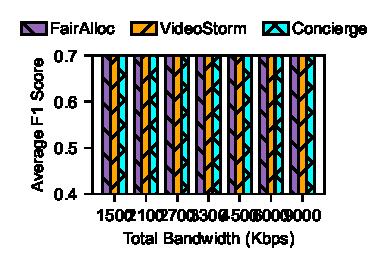
\includegraphics{./resources/concierge-perf.pdf}
    %     \caption{Tingkah Laku Sistem}\label{fig:resource_alloc_tes}
    % \end{figure}
% \begin{algorithm}
%     \caption{An algorithm with caption}\label{alg:cap}
%     \begin{algorithmic}
%     \Require $n \geq 0$
%     \Ensure $y = x^n$
%     \State $y \gets 1$
%     \State $X \gets x$
%     \State $N \gets n$
%     \While{$N \neq 0$}
%     \If{$N$ is even}
%         \State $X \gets X \times X$
%         \State $N \gets \frac{N}{2}$  \Comment{This is a comment}
%     \ElsIf{$N$ is odd}
%         \State $y \gets y \times X$
%         \State $N \gets N - 1$
%     \EndIf
%     \EndWhile
%     \end{algorithmic}
%     \end{algorithm}

